\documentclass[main.tex]{subfiles}
\begin{document}
	
	\chapter{Perception}
		\chapterauthor{Author}
		
		\section{General}
		The main changes and improvements upon the status presented at milestone 1 are the following: Perception now runs inside an actionserver, in contrast to 				plain robosherlock. Additionally, Caffe is now used for feature extraction, and KNN is used for the classification of detected objects. We also recorded 				image data of objects available to us, which were then used for classification purposes.
		
		\section{Actionserver}
			\subsection{Interfaces}
			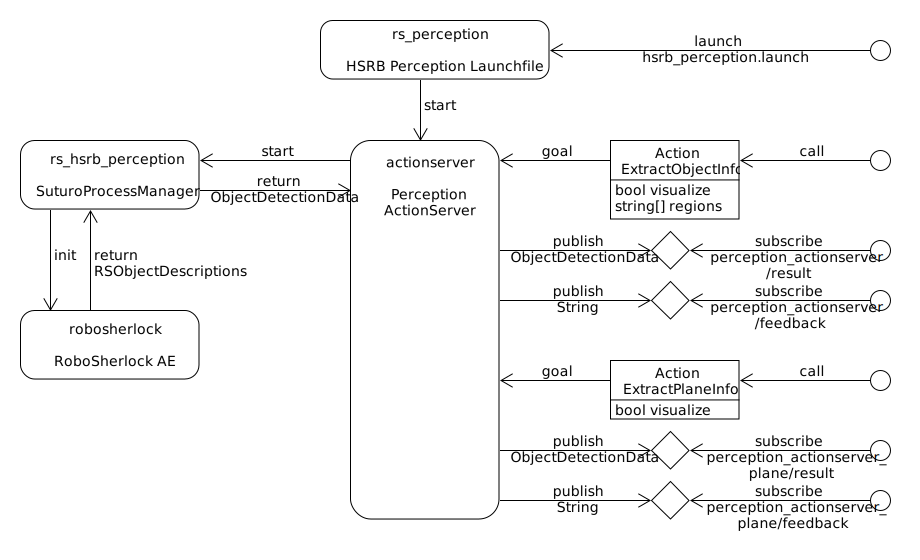
\includegraphics[width=\textwidth]{../architecture/perception_architecture/perception.pdf}
			
			\subsection{Packages}
			\subsubsection{actionserver}
			Implements the "ExtractObjectInfo" and "ExtractPlaneInfo" action servers and the corresponding action clients.
			Internally the "SuturoProcessManager" from "rs\_hsrb\_perception" is used to communicate with RoboSherlock.
			The action server invokes "SuturoProcessManager::run()" with the given parameters. 

			\subsubsection{rs\_perception}
			Includes launch-, configuration- and analysis descriptor files.
			In order to start the perception action servers you have to call:\\
			"roslaunch rs\_perception hsrb\_perception.launch"\\
			To convert published URDFs to YAML run: "region\_filter\_setup.py" (originally from Suturo1819).\\
			Generated YAML map descriptors must be placed in the "config" folder.

			\subsubsection{rs\_hsrb\_perception (forked from suturo1819)}
			Implements a RoboSherlock process manager "SuturoProcessManager".
			The manager gets called from the "actionserver" and executes the selected pipeline once.
			
			In order to perceive objects that are placed on the ground, the SuturoRegionFilter gets reconfigured
			to disable the region filtering. Set the region parameter to \{ "robocup\_default" \} to enable this feature.

		\section{Classification}
		
		\section{Recording of images}  

\end{document}
